\subsection{Constraints}
\label{subsec:constraints}
Some of the system limitations that we discovered during the process of developing the system context are shown in Fig. 4's constraints diagram. The system is required to schedule traffic for autonomous vehicles at the intersection, which it does by using the concept of ROW (right of way). The system determines the order in which vehicles can proceed through the intersection based on predefined rules and priorities. For our system, we consider four possible ROWs. The following are the five system constraints that we consider for our system:
\begin{enumerate}
    \item The time extension for public transport is only possible when it has the same ROW as the one scheduled.
    \item At a given time only one ROW is allowed to execute.
    \item The vehicle can connect to the infrastructure when it is in a defined range. 
    \item The is a defined max load that the infrastructure can handle at a given time.
    \item The transfer rate should be less than the defined limit. 
    
\end{enumerate}
\begin{figure}[ht]
    \centering
    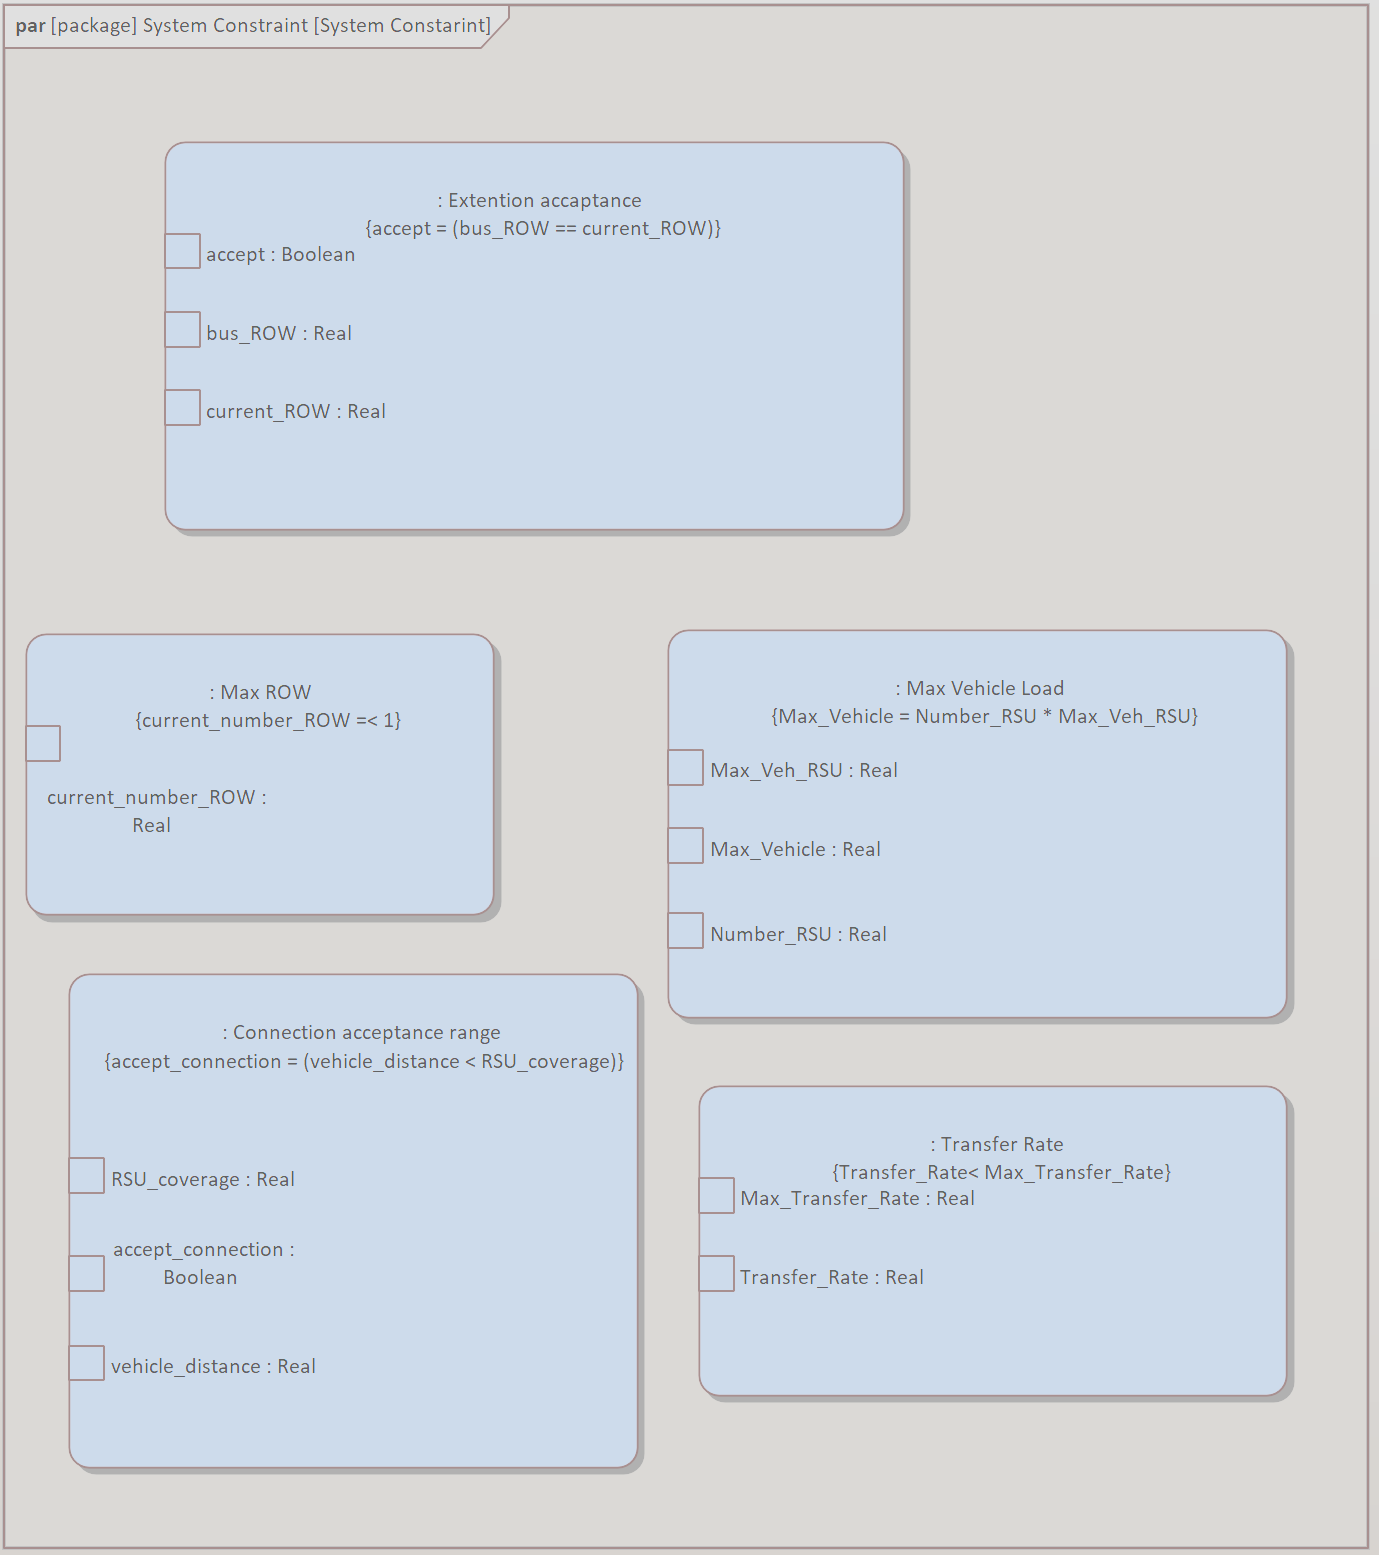
\includegraphics[width=0.4\textwidth]{images/system_constraint.png}
    \caption{System Constraint Diagram}
    \label{img:system_constraints}
\end{figure}